\section{Estensioni e originalità}
\label{cap:extensions-and-originalities}

\noindent Oltre all'implementazione richiesta dalla consegna
dell'homework, abbiamo deciso di esplorare un altro algoritmo per il problema del taglio minimo.

\subsection{Algoritmo di Karger \& Stein}
\label{sub:karger-stein-algorithm}

L'algortimo di Karger \& Stein è una variante migliorata del semplice algoritmo di Karger. Come abbiamo osservato nella sezione TODO, la probabilità che l'algoritmo di Karger non scelga un arco del taglio minimo tende a diminuire man mano che l'algoritmo durante le iterazione scegli l'arco dove contrarre il grafo. Per questo motico l'algoritmo di Karger \& Stein svolge le prime iterazioni (dove la probabilità di non scelre un arco del min-cut) come l'algoritmo di Karger, mentre le "ultime" iterazioni vengono ripetute più volte con la speranza che qaulcuna di queste non becchi proprio l'arco del min-cut. \\

\noindent Ora supponiamo di volere contrarre gli archi tra n vertici e k vertici in 2 iterazioni di karger normale distinte. Possiamo scegliere a questo punto k in modo da avere una probabilità di successo (ossia di trovare il min-cut) di $\dfrac{1}{2}$. Dunque in questo modo sappiamo che una delle sue esecuzioni indipendenti di Karger avrà successo. Prendiamo quella che ha successo e rieseguiamo tale procedura per il miglior grafo ricavato in una di queste 2 escuzioni. \\

\noindent Se scegliamo k (ossia il numero di iterazioni iniziali) pari a:
$$ k = \dfrac{n}{\sqrt{2}} + 1$$
che equivale a circa il 70\% dei nodi $n$ del grafo rimanenti da contrarre (o equivalentemente abbiamo contratto il 30\% dei nodi $n$ del grafo) a questo punto otteniamo la probabilità desiderata, infatti:

$$ = (1 - \frac{2}{n}) * (1 - \frac{2}{n-1}) * (1 - \frac{2}{n-2}) * ... * (1 - \frac{2}{k+1}) $$

$$ = \dfrac{(1 - \frac{2}{n}) ... (1 - \frac{2}{3})}{(1 - \frac{2}{k}) ... (1 - \frac{2}{3})} = \dfrac{{k\choose 2}^{-1}} {{k\choose 2}^{-1}} = \dfrac{k(k-1)}{n(n-1)}$$

\noindent se inseriamo ora $$ k = \dfrac{n}{\sqrt{2}} + 1$$ otteniamo:
$$ ... = \dfrac{k(k-1)}{n(n-1)} = \dfrac{(\dfrac{n}{\sqrt{2}} + 1) (\dfrac{n}{\sqrt{2}} + 1 - 1)}{n(n-1)} = (\dfrac{\dfrac{n^2}{2} + \dfrac{n}{\sqrt{2}}}{n^2 - n}) \geq \dfrac{1}{2}$$

\noindent come desiderato.\\

\noindent Pertanto l'algoritmo di Karger \& Stein è così formato:
\begin{enumerate}
    \item \textbf{Step 1}: Se $n <= 6$ esegui l'algoritmo di Karger normale stimando il parametro k come visto sopra;
    \item \textbf{Step 2a}: Altrimenti esegui 2 esecuzioni indipendenti di Karger fino a raggiungere $\frac{n}{\sqrt{2}}$ vertici;
    \item \textbf{Step 2b}: Prendi il miglior risultato di queste due esecuzioni e riesegui la seguente procedura.
\end{enumerate}

Il listato \ref{listing:karger&stein} contiene la nostra implementazione di questo algoritmo.


\begin{listing}[!ht]
\begin{minted}{c++}
// kager_stein.h
[[nodiscard]] size_t fast_min_cut(const std::shared_ptr<AdjacencyMapGraph>& graph)
noexcept {
    const size_t n = graph->size();

    // Step 1
    if (n <= 6) {
        const size_t k = utils::estimate_iterations_karger(n);
        return karger(graph, k);
    }

    // Step 2a
    const size_t t =
        static_cast<size_t>(std::ceil((static_cast<double>(n) / std::sqrt(2))));

    auto g1 = full_contraction(graph, t);
    auto g2 = full_contraction(graph, t);


    // Step 2b
    return std::min(fast_min_cut(std::move(g1)), fast_min_cut(std::move(g2)));
}
\end{minted}
\caption{Implementazione dell'algoritmo di Karger \& Stein.}
\label{listing:karger&stein}
\end{listing}


\subsubsection{Successo con alta probabilità e complessità}
\label{sub:karger-stein-success-whp}

Per cominciare calcoliamo il nuovo tempo di esecuzione per una singola iterazione:
$$T(n) = 2T(\dfrac{n}{\sqrt{2}}) + O(n^2) $$
Dal Teorema Master deduciamo quindi che $T(n) = O(n^2 \log{n})$\\

\noindent Possiamo ora quindi scrivere una relazione ricorrente per il successo in probabilità. Sappiamo che la probabilità di successo nelle contrazioni da n a $\dfrac{n}{\sqrt{2}} + 1$ non è più piccola di $\frac{1}{2}$, dunque:
$$P(n) \geq 1-(1- \frac{1}{2}P(\dfrac{n}{\sqrt{2}}))^2$$
A questo punto si può vedere che usando l'induzione: $P(n)= \Omega(\frac{1}{\log{n}}) $. Dunque se facciamo $O(\log^2{n})$ esecuzioni la probabilità di successo e almeno $1-\dfrac{1}{poly(n)}$. Dunque, il tempo di esecuzione totale di questo algoritmo è di:

$$O(n^2 \log^3{n})$$

\subsection{Confronto con KargerMinCut}

\noindent L'algoritmo di Karger \& Stein è nettamente più veloce rispetto all'algoritmo di Karger, com'è possibile vedere in figura \ref{fig:karger-vs-karger-stein}. Basti pensare che eseguire KargerMinCut su tutti e 40 le istanze del dataset richiede circa 2 ore sul computer usato per i benchmark, mentre KargerSteinMinCut richiede circa 2 minuti. Per le istanze a disposizione, l'algoritmo di Karger \& Stein è quindi circa 60 volte migliore di Karger.

\begin{figure}[H]
    \centering

    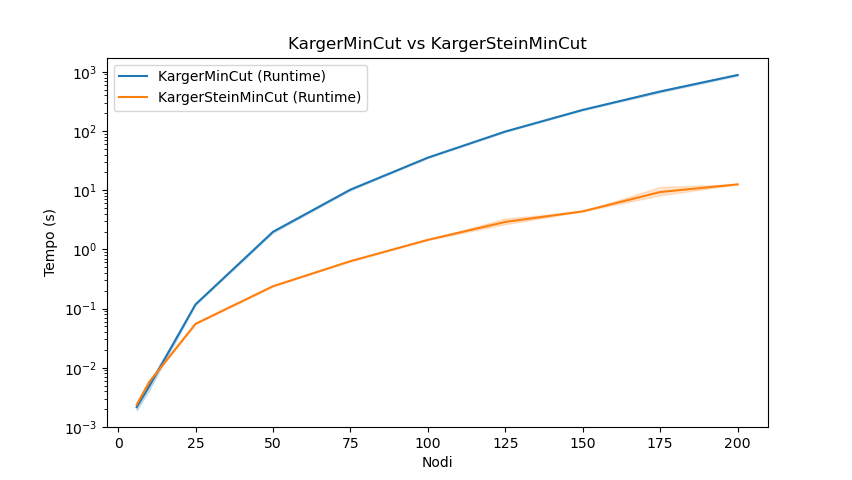
\includegraphics[width=0.9\textwidth]{./images/karger_vs_karger_stein - log.png}

    \caption{Confronto del tempo di esecuzione (in secondi) di Karger \& Stein rispetto a Karger. Grafico in scala logaritmica.}
    \label{fig:karger-vs-karger-stein}
\end{figure}

\subsection{Confronto con KargerMinCutTimeout}

\noindent Chiaramente la differenza di tempi di esecuzione i due algoritmi si riduce se si confronta Karger \& Stein con Karger con timeout $T = 2$ minuti . Come si evince dalla linea piatta in alto a destra di Figura \ref{fig:karger-timeout-vs-karger-stein}, le istanze con più di 150 nodi richiederebbero più di 2 minuti di esecuzioni, quindi l'algoritmo di Karger viene terminato prematuramente.

\begin{figure}[H]
    \centering

    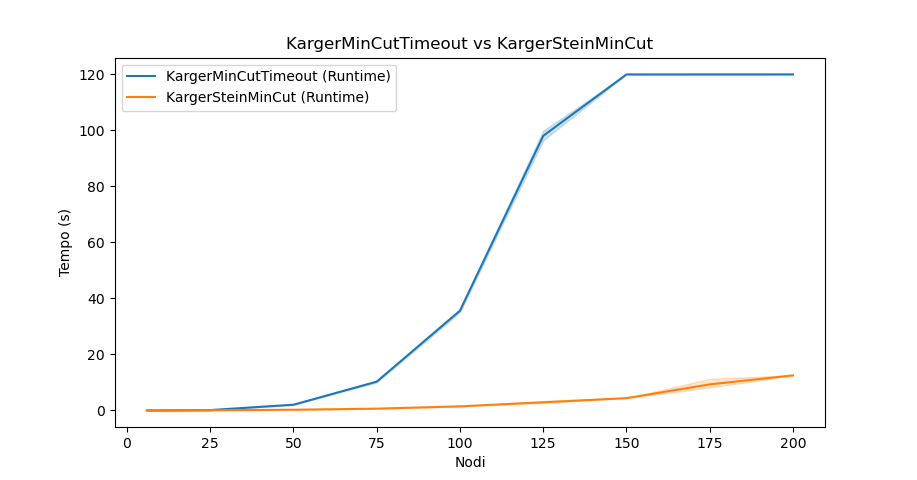
\includegraphics[width=0.9\textwidth]{./images/karger_timeout_vs_karger_stein.png}

    \caption{Confronto del tempo di esecuzione (in secondi) di Karger \& Stein rispetto a Karger con timeout $T = 2 \text{minuti}$.}
    \label{fig:karger-timeout-vs-karger-stein}
\end{figure}

% \ref{table:karger-stein-running-time}
